\documentclass[11pt,a4paper]{article}

\newcommand{\docshorttitle}{HomeSense --- Technical Report}
% Shared preamble for the HomeSense project documents.
% Compiled with Tectonic (XeTeX). See build.ps1.

\usepackage[a4paper,margin=25mm,headheight=15pt]{geometry}
\usepackage{fontspec}
\usepackage{amsmath}
\usepackage{amssymb}   % provides \square, used for checklist items
\usepackage{microtype}
\usepackage{booktabs}
\usepackage{tabularx}
\usepackage{longtable}
\usepackage{array}
\usepackage{xcolor}
\usepackage{graphicx}
\usepackage{enumitem}
\usepackage{fancyhdr}
\usepackage{titlesec}
\usepackage{caption}
\usepackage{listings}
\usepackage{tikz}
\usetikzlibrary{positioning,arrows.meta,calc,shapes.geometric,fit,backgrounds}
\usepackage[hidelinks]{hyperref}

% --- typography -------------------------------------------------------------
\setmainfont{Times New Roman}[
  BoldFont={Times New Roman Bold},
  ItalicFont={Times New Roman Italic},
  BoldItalicFont={Times New Roman Bold Italic}
]
\setmonofont{Consolas}[Scale=0.86]

\linespread{1.08}
\setlength{\parskip}{0.6em}
\setlength{\parindent}{0pt}
\setlist{itemsep=0.15em,topsep=0.35em,parsep=0pt}

% --- colours ----------------------------------------------------------------
\definecolor{rule}{HTML}{9AA5B1}
\definecolor{codebg}{HTML}{F5F7F9}
\definecolor{codekw}{HTML}{0B5FA5}
\definecolor{codestr}{HTML}{1B7F3B}
\definecolor{codecom}{HTML}{6B7280}
\definecolor{accent}{HTML}{00696D}
\definecolor{boxbg}{HTML}{F0F4F6}

% --- headings ---------------------------------------------------------------
\titleformat{\section}{\large\bfseries}{\thesection}{0.7em}{}
\titleformat{\subsection}{\normalsize\bfseries}{\thesubsection}{0.7em}{}
\titleformat{\subsubsection}{\normalsize\itshape}{\thesubsubsection}{0.7em}{}
\titlespacing*{\section}{0pt}{1.8em}{0.6em}
\titlespacing*{\subsection}{0pt}{1.2em}{0.4em}

% --- headers and footers ----------------------------------------------------
\pagestyle{fancy}
\fancyhf{}
\renewcommand{\headrulewidth}{0.4pt}
\fancyhead[L]{\small\textsc{\docshorttitle}}
\fancyhead[R]{\small SCS 3311}
\fancyfoot[C]{\small\thepage}

% --- tables -----------------------------------------------------------------
\renewcommand{\arraystretch}{1.25}
\newcolumntype{L}[1]{>{\raggedright\arraybackslash}p{#1}}
\captionsetup{font=small,labelfont=bf,skip=6pt}

% --- inline code ------------------------------------------------------------
% Handles underscores without manual escaping, so field names such as
% max_on_duration can be written naturally.
\newcommand{\code}[1]{\texttt{\small #1}}

% --- code listings ----------------------------------------------------------
\lstdefinestyle{project}{
  backgroundcolor=\color{codebg},
  basicstyle=\ttfamily\scriptsize,
  keywordstyle=\color{codekw}\bfseries,
  stringstyle=\color{codestr},
  commentstyle=\color{codecom}\itshape,
  numberstyle=\tiny\color{codecom},
  breaklines=true,
  breakatwhitespace=true,
  captionpos=b,
  frame=single,
  rulecolor=\color{rule},
  framesep=5pt,
  xleftmargin=8pt,
  xrightmargin=4pt,
  showstringspaces=false,
  tabsize=2,
  columns=fullflexible,
  keepspaces=true,
  upquote=true,
}
\lstset{style=project}

\lstdefinelanguage{Kotlin}{
  keywords={package,as,typealias,class,this,super,val,var,fun,for,while,do,null,
    true,false,is,in,throw,return,break,continue,object,if,else,when,try,catch,
    finally,for,do,while,interface,data,sealed,override,private,public,internal,
    suspend,operator,companion,by,import,enum,const},
  sensitive=true,
  comment=[l]{//},
  morecomment=[s]{/*}{*/},
  morestring=[b]",
}

% --- callout box ------------------------------------------------------------
\newcommand{\keypoint}[1]{%
  \par\vspace{0.4em}%
  \noindent\begin{tikzpicture}
    \node[draw=rule,fill=boxbg,line width=0.4pt,rounded corners=2pt,
          inner sep=9pt,text width=\dimexpr\textwidth-24pt\relax,align=justify]
      {#1};
  \end{tikzpicture}%
  \par\vspace{0.4em}%
}

% --- title page -------------------------------------------------------------
\newcommand{\titlepagestandard}[2]{%
\begin{titlepage}
\centering
\vspace*{2.2cm}

{\Large\scshape University of Colombo School of Computing\par}
\vspace{0.4cm}
{\large SCS 3311 --- Mobile Application Design and Development\par}
\vspace{0.3cm}
{\large Mini-Project\par}

\vspace{2.4cm}
{\rule{\textwidth}{0.8pt}}
\vspace{0.7cm}

{\LARGE\bfseries HomeSense\par}
\vspace{0.5cm}
{\Large Smart Home Monitoring and Control System\par}
\vspace{0.7cm}
{\large #1\par}

\vspace{0.7cm}
{\rule{\textwidth}{0.8pt}}

\vspace{2.4cm}

{\large\bfseries Group Members\par}
\vspace{0.6cm}

\begin{tabular}{@{}L{4.6cm}L{3.1cm}L{6.6cm}@{}}
\toprule
\textbf{Name} & \textbf{Index number} & \textbf{Module} \\
\midrule
R.L. Weerasinghe & 23002204 & Synchronisation, simulator and safety worker \\
W.T. Mahagamage  & 23001038 & Device profiles, control interface and reporting \\
D.M. Isakya      & 23000643 & Floor representation and grid mapping \\
\bottomrule
\end{tabular}

\vfill
{#2\par}
\vspace{0.8cm}
\end{titlepage}
}


\begin{document}

\titlepagestandard{Technical Report}{\large August 2026}

\tableofcontents
\thispagestyle{fancy}
\newpage

% ============================================================================
\section{Introduction}

The system comprises an Android client, a web-based hardware simulator and a
server-side worker process, all communicating through a Firebase Realtime
Database. Users manage multiple floor plans, place devices of differing
capabilities onto an abstract grid, and control them from the mobile client.
The worker enforces safety policy independently of the client.

This report covers the three areas specified for assessment: the synchronising
mechanism, the floor representation, and the simulator operations. Architecture,
verification and limitations are addressed within those sections or in the
appendices.

\subsection{Scope of the implementation}

All functional requirements of the specification are implemented. Appendix
\ref{app:traceability} maps each requirement to the source file implementing it,
the test verifying it, and the point in the demonstration at which it is shown.

% ============================================================================
\section{Synchronising mechanism}

\subsection{State model}

The system distinguishes between three related but separate facts about every
controllable point in the house. Rather than storing a single boolean per
switch, each slot stores three, as shown in Table \ref{tab:threefields}.

\begin{table}[h]
\centering
\caption{The three state fields and the component responsible for each}
\label{tab:threefields}
\begin{tabular}{@{}L{3.2cm}L{5.6cm}L{5.4cm}@{}}
\toprule
\textbf{Field} & \textbf{Meaning} & \textbf{Written by} \\
\midrule
\code{desiredState}  & The state requested by the user & Mobile client, and the worker for cut-offs and schedules \\
\code{reportedState} & The state the hardware confirms & Simulator \\
\code{status}        & The reconciled value presented in the interface & Worker \\
\bottomrule
\end{tabular}
\end{table}

A single boolean cannot distinguish between a state that has been requested, a
state that is actually in effect, and the system's confidence in that
information. Three fields make the distinction explicit, and this is what allows
the \code{ERROR} and \code{DISCONNECTED} states to carry meaning:

\begin{itemize}
  \item \code{ERROR} is raised only when \code{desiredState} and
        \code{reportedState} disagree for longer than a tolerance window of ten
        seconds. A brief disagreement is expected during normal operation, as it
        represents a command in transit.
  \item \code{DISCONNECTED} is raised only when a device's heartbeat is older
        than fifteen seconds. It takes precedence over all other states. Where
        no report has been received, presenting \code{OFF} would express an
        assumption as though it were an observation.
\end{itemize}

\subsection{Choice of database}

Firebase Realtime Database was selected in preference to Cloud Firestore for two
reasons.

First, Realtime Database supports per-child listeners. Toggling a single slot
produces one \code{onChildChanged} callback carrying that device, rather than a
retransmission of the whole \code{/devices} subtree. For a grid of independently
toggled slots this materially affects both latency and data volume.

Second, Realtime Database provides \code{onDisconnect()}, which allows the
server to record a client's disappearance. Without it, absence would have to be
inferred by each observer independently.

Firestore's document-level listener granularity and higher write latency are
less suited to this access pattern. The cost of the choice is the absence of
meaningful query support and a denormalised tree that must be kept consistent by
convention. This is acceptable here because the tree is small, its shape is
fixed, and it is documented in full in the project's data contract.

\subsection{Propagation of a state change}

Figure \ref{fig:sequence} traces a single toggle from the user's tap to the
confirmed status.

\begin{figure}[htbp]
\centering
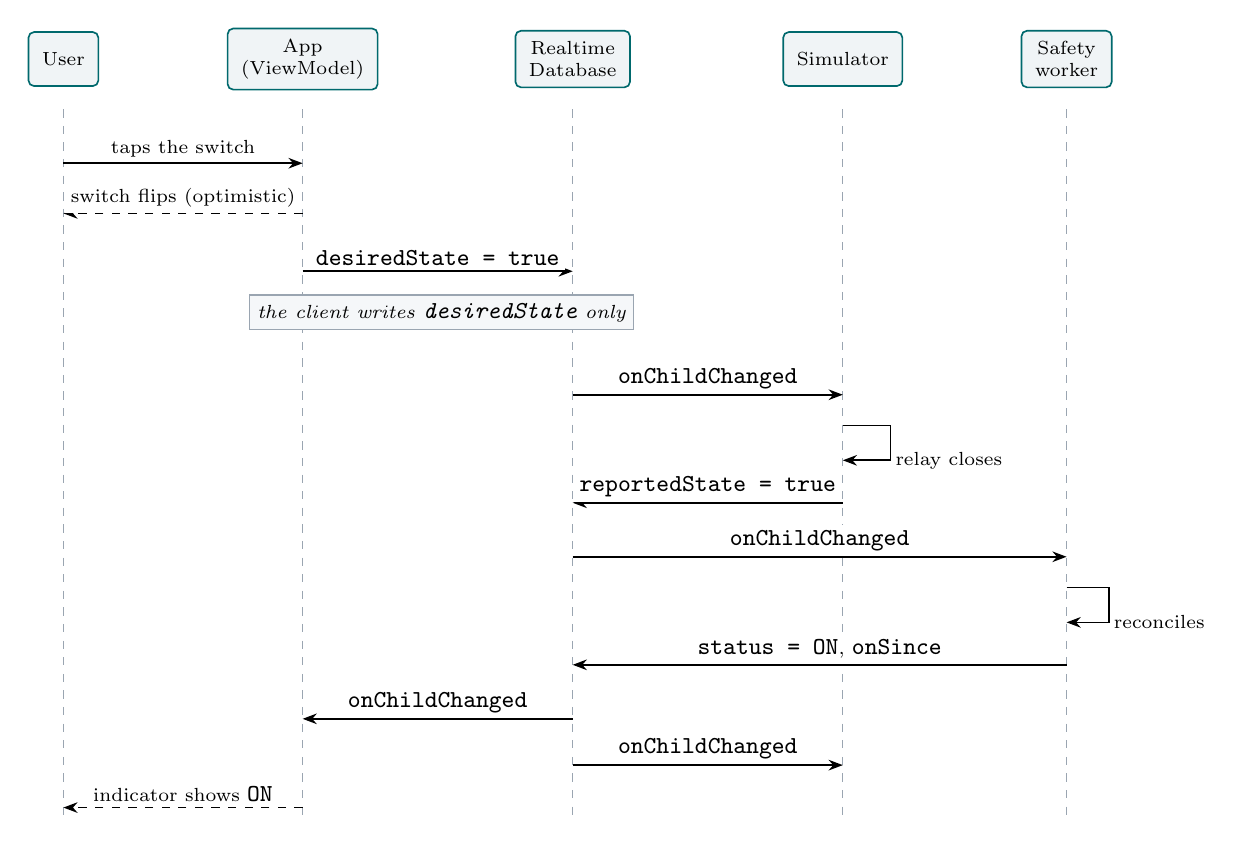
\begin{tikzpicture}[
    scale=0.98,
    every node/.style={transform shape},
    font=\scriptsize,
    lifeline/.style={draw=rule,dashed,line width=0.5pt},
    actor/.style={draw=accent,fill=boxbg,line width=0.6pt,rounded corners=2pt,
                  inner xsep=5pt,inner ysep=4pt,minimum height=7mm,align=center},
    msg/.style={-{Stealth[length=1.8mm]},line width=0.6pt},
    ret/.style={-{Stealth[length=1.8mm]},line width=0.6pt,dashed},
    note/.style={draw=rule,fill=codebg,line width=0.4pt,inner sep=3pt,
                 align=center,font=\scriptsize\itshape},
    % Message labels sit on an opaque background so that an arrow spanning
    % several participants does not collide with the lifelines it crosses.
    every node/.append style={fill=white,inner sep=2pt}
  ]

  % participants
  \node[actor] (hU) at (0,0)    {User};
  \node[actor] (hA) at (3.1,0)  {App\\(ViewModel)};
  \node[actor] (hD) at (6.6,0)  {Realtime\\Database};
  \node[actor] (hS) at (10.1,0) {Simulator};
  \node[actor] (hW) at (13.0,0) {Safety\\worker};

  % lifelines
  \draw[lifeline] (0,-0.65)    -- (0,-9.9);
  \draw[lifeline] (3.1,-0.65)  -- (3.1,-9.9);
  \draw[lifeline] (6.6,-0.65)  -- (6.6,-9.9);
  \draw[lifeline] (10.1,-0.65) -- (10.1,-9.9);
  \draw[lifeline] (13.0,-0.65) -- (13.0,-9.9);

  % request
  \draw[msg] (0,-1.35) -- node[above]{taps the switch} (3.1,-1.35);
  \draw[ret] (3.1,-2.0) -- node[above]{switch flips (optimistic)} (0,-2.0);
  \draw[msg] (3.1,-2.75) -- node[above]{\code{desiredState = true}} (6.6,-2.75);

  \node[note,anchor=north] at (4.9,-3.05)
    {the client writes \code{desiredState} only};

  % hardware responds
  \draw[msg] (6.6,-4.35) -- node[above]{\code{onChildChanged}} (10.1,-4.35);
  \draw[msg] (10.1,-4.75) -- ++(0.62,0) -- ++(0,-0.45)
    node[right,inner sep=1.5pt]{relay closes} -- ++(-0.62,0);
  \draw[msg] (10.1,-5.75) -- node[above]{\code{reportedState = true}} (6.6,-5.75);

  % worker reconciles
  \draw[msg] (6.6,-6.45) -- node[above]{\code{onChildChanged}} (13.0,-6.45);
  \draw[msg] (13.0,-6.85) -- ++(0.55,0) -- ++(0,-0.45)
    node[right,inner sep=1.5pt]{reconciles} -- ++(-0.55,0);
  \draw[msg] (13.0,-7.85) -- node[above]{\code{status = ON}, \code{onSince}} (6.6,-7.85);

  % fan-out
  \draw[msg] (6.6,-8.55) -- node[above]{\code{onChildChanged}} (3.1,-8.55);
  \draw[msg] (6.6,-9.15) -- node[above]{\code{onChildChanged}} (10.1,-9.15);
  \draw[ret] (3.1,-9.7) -- node[above]{indicator shows \code{ON}} (0,-9.7);

\end{tikzpicture}
\caption{Propagation of a single toggle. The client requests a state; the
simulator confirms it; the worker publishes the reconciled status. The
indicator reflects confirmation rather than intent.}
\label{fig:sequence}
\end{figure}

Three properties follow from this arrangement.

\subsubsection{Updates require no manual refresh}

The repository interface exposes no \code{refresh()}, \code{reload()} or
\code{fetch()} method, because none is required. The device list is a
\code{StateFlow} supplied directly by database child listeners, so a change
originating in the simulator, the worker or a second client arrives as a
callback and causes recomposition.

The repository tests demonstrate this by emitting a change on the source and
asserting that the flow carries it, without any call into the repository.

\subsubsection{Toggles are optimistic but reconciled}

The switch position changes immediately, since waiting for a network round trip
degrades the perceived responsiveness of the interface. However, the client
writes only \code{desiredState} and cannot itself operate a relay. The
optimistic position is therefore held for a maximum of four seconds; if
\code{reportedState} has not followed within that window, the control reverts
and the user is informed.

Four seconds was chosen to sit between a normal round trip and the worker's
ten-second \code{ERROR} threshold, so that the user is notified shortly before
the status indicator changes.

\subsubsection{The write separation is enforced by the database}

In Realtime Database a \code{.write} grant propagates to all descendants of the
node at which it is declared and cannot be withdrawn at a lower level, so a
nested \code{.write: false} has no effect. Validation rules, by contrast, do
restrict client writes, and the Admin SDK bypasses validation entirely.

The security rules use this asymmetry. The fields \code{status}, \code{link},
\code{onSince} and \code{mismatchSince} carry validators that accept a write
only when the value is unchanged:

\begin{lstlisting}[language=,caption={Immutability validator applied to the
status field in \code{database.rules.json}},label={lst:rules}]
"status": {
  ".validate": "(newData.val() == 'ON'    || newData.val() == 'OFF' ||
                 newData.val() == 'ERROR' || newData.val() == 'DISCONNECTED')
                && ((!data.exists() && newData.val() == 'DISCONNECTED')
                    || newData.val() == data.val())"
}
\end{lstlisting}

\keypoint{An authenticated client cannot publish a status value, clear an
\code{ERROR}, or suppress a \code{DISCONNECTED} state, while the worker writes
these fields without restriction. A limitation of this approach is documented in
Appendix \ref{app:limitations}.}

\subsection{Authentication and tenancy}

Synchronisation is only meaningful once it is established whose data is being
synchronised. Two questions are answered separately.

\textbf{Identity} is handled by Firebase Authentication with email and password.
An anonymous session is also offered so the application can be tried before
registering; it is upgraded in place with \code{linkWithCredential}, which
preserves the account identifier, so a guest who later registers keeps the
household, history and alerts accumulated in the meantime.

\textbf{Tenancy} is separate. An account belongs to zero or more households, and
a household records its members at \code{homes/\$homeId/members}. Every read and
write rule consults that record, so a household is confined to the people
admitted to it. Members are admitted in one of two ways: by creating the
household, which makes the creator its owner, or by redeeming an invite code.

The invite is verified by the database rather than trusted from the client. The
joining member writes the code into its own membership record, and the rule
accepts the write only if that code exists under \code{/invites}, names this
household, and has not expired. There is no read rule on the invite collection
itself, only on an individual code, so a code can be redeemed when already known
but the collection cannot be enumerated.

Two roles are distinguished. Any member may operate devices and edit ordinary
schedules; only the owner may add or remove devices, configure
\code{max\_on\_duration}, and manage membership. Safety configuration is
reserved to the owner because altering a cut-off changes the protection applied
to everyone in the house.

\keypoint{Three consequences of introducing sessions had to be handled
explicitly rather than emerging on their own. The data layer subscribes through
the active household as a flow, so signing out tears down every listener rather
than leaving them attached to a household the session is no longer entitled to.
The local cache is cleared when the account changes, since Room holds usage
history and alerts that would otherwise be visible to the next person to sign in
on the same device. And push notifications are published to a topic named after
the household rather than to a single shared topic, which would have delivered
every family's cut-off alerts to every installation.}

\subsection{Offline behaviour and usage logging}

Realtime Database disk persistence is enabled, so the most recently received
tree is available locally and the first frame after a cold start displays real
data rather than a loading indicator. A Room database mirrors floors, device
layout, alerts and the usage log. Live device status is deliberately excluded
from this mirror: an outdated \code{ON} indicator is more misleading than an
honest \code{DISCONNECTED}.

Usage events are append-only. Each is written at the moment of transition by
whichever component caused it, and usage is never reconstructed by comparing
successive snapshots. Reconstruction by comparison would omit every transition
occurring while the client was closed, which is precisely the period the safety
worker exists to cover.

% ============================================================================
\section{Floor representation}

\subsection{Coordinate model}

A device represents one physical node, occupying one grid cell with one network
connection and one heartbeat. Its position is stored as integer cell
coordinates rather than pixel offsets, so that a plan renders consistently
across screen sizes and orientations.

Translation between cell coordinates and screen coordinates is confined to a
single class, \code{GridMapper}, which has no Android dependencies and is
therefore testable as a plain JVM unit. Sixteen tests cover the cell-to-pixel
round trip for every cell, taps falling on the letterbox margins, taps on cell
boundaries and plan edges, degenerate zero-sized canvases, and the property that
a given cell resolves identically under phone and tablet geometry.

Because a plan has a fixed aspect ratio and the available canvas generally does
not, the plan is fitted within the canvas with its ratio preserved, leaving
margins on two sides, as illustrated in Figure \ref{fig:letterbox}. All cell
arithmetic is performed relative to the fitted rectangle rather than the raw
canvas bounds; otherwise the grid would stretch with the window and device
positions would drift.

\begin{figure}[htbp]
\centering
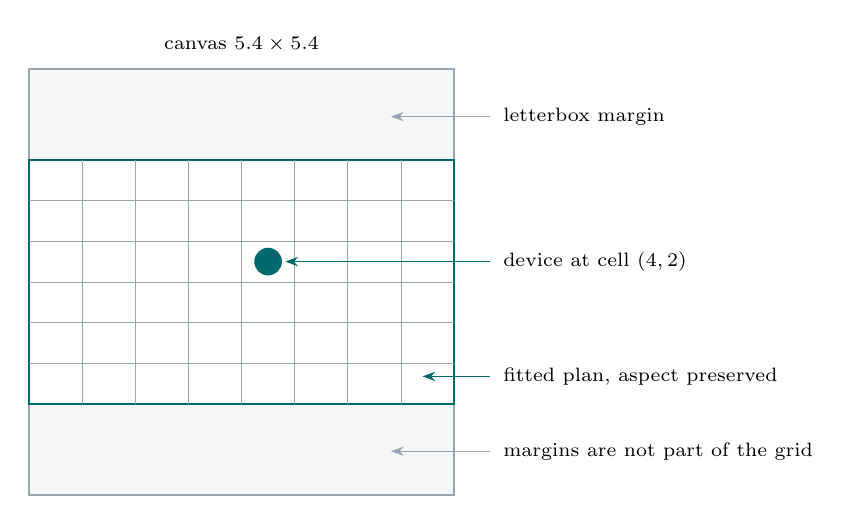
\begin{tikzpicture}[font=\footnotesize]

  % canvas
  \draw[draw=rule,line width=0.7pt] (0,0) rectangle (5.4,5.4);
  \node[font=\scriptsize,anchor=south] at (2.7,5.5) {canvas $5.4 \times 5.4$};

  % letterbox margins
  \fill[codebg] (0,4.25) rectangle (5.4,5.4);
  \fill[codebg] (0,0) rectangle (5.4,1.15);
  \draw[draw=rule,line width=0.7pt] (0,0) rectangle (5.4,5.4);

  % fitted plan
  \draw[draw=accent,line width=0.9pt,fill=white] (0,1.15) rectangle (5.4,4.25);

  % grid
  \foreach \i in {1,...,7} \draw[rule,line width=0.3pt]
    ({\i*5.4/8},1.15) -- ({\i*5.4/8},4.25);
  \foreach \j in {1,...,5} \draw[rule,line width=0.3pt]
    (0,{1.15+\j*3.1/6}) -- (5.4,{1.15+\j*3.1/6});

  % a placed device
  \fill[accent] ({4.5*5.4/8},{1.15+3.5*3.1/6}) circle (5pt);

  \node[font=\scriptsize,anchor=west] at (5.9,4.8) {letterbox margin};
  \draw[-{Stealth[length=1.6mm]},rule] (5.85,4.8) -- (4.6,4.8);

  \node[font=\scriptsize,anchor=west] at (5.9,{1.15+3.5*3.1/6})
    {device at cell $(4,2)$};
  \draw[-{Stealth[length=1.6mm]},accent] (5.85,{1.15+3.5*3.1/6})
    -- ({4.5*5.4/8+0.22},{1.15+3.5*3.1/6});

  \node[font=\scriptsize,anchor=west] at (5.9,1.5)
    {fitted plan, aspect preserved};
  \draw[-{Stealth[length=1.6mm]},accent] (5.85,1.5) -- (5.0,1.5);

  \node[font=\scriptsize,anchor=west] at (5.9,0.55)
    {margins are not part of the grid};
  \draw[-{Stealth[length=1.6mm]},rule] (5.85,0.55) -- (4.6,0.55);

\end{tikzpicture}
\caption{A 4:3 plan fitted into a square canvas. Cell arithmetic is performed
relative to the fitted rectangle, so a tap on the margin resolves to no cell
rather than to an out-of-range coordinate.}
\label{fig:letterbox}
\end{figure}

\subsection{Representation of plans}

The specification calls for an abstract and simple mapping. Plans are
accordingly declared as geometry --- rooms, doorways and windows in a unit-less
coordinate space, defined in \code{FloorPlanSpec} --- and rendered using the
Compose \code{Canvas} API.

This approach has three advantages over bundled raster images. Rendering remains
sharp at any screen density, with no bitmap scaling. The aspect ratio is exact,
which makes the fitting calculation exact. And since the plans are original
work, no third-party image licence needs to be tracked or attributed.

Three sample plans are supplied (ground floor, first floor and an annex),
together with a blank grid. A floor record stores only the identifier of its
plan, so changing a floor's layout does not affect the devices placed on it.

\subsection{Visual encoding}

Device markers encode kind through shape and status through fill pattern, as
listed in Table \ref{tab:markers}.

\begin{table}[h]
\centering
\caption{Visual encoding of device kind and operational status}
\label{tab:markers}
\begin{tabular}{@{}L{4.0cm}L{9.5cm}@{}}
\toprule
\textbf{Attribute} & \textbf{Encoding} \\
\midrule
Outlet             & Circle \\
Multi-switch       & Square, with one indicator per addressable slot \\
Camera             & Body-and-lens outline \\
\midrule
\code{ON}          & Solid fill \\
\code{OFF}         & Plain outline \\
\code{ERROR}       & Outline with a cross \\
\code{DISCONNECTED}& Dashed outline \\
\bottomrule
\end{tabular}
\end{table}

No state is conveyed by colour alone anywhere in the application. Status is
always presented as colour together with an icon and a text label. This is
required for accessibility, and it also ensures the interface remains legible
when projected.

Where a multi-switch unit has slots in differing states, its marker shows the
most severe of them, so that a fault on one channel is not concealed by two
functioning channels.

\subsection{Multi-switch units}

The specification requires that a multi-switch unit be mapped to a single
entity. The data model enforces this: \code{Device} holds a list of \code{Slot}
values, so a five-gang plate is one device identifier, one grid cell and one
heartbeat, with five independently addressable slots and a master control that
addresses each in sequence. No code path produces more than one device from a
single unit.

\begin{lstlisting}[language=Kotlin,caption={The device and slot relationship,
abridged from \code{domain/model/Device.kt}},label={lst:device}]
data class Device(
    val id: String = "",
    val gridX: Int = 0,
    val gridY: Int = 0,
    val kind: DeviceKind = DeviceKind.OUTLET,
    val slots: List<Slot> = emptyList(),   // 1 for an outlet, 2..6 for a gang box
)
\end{lstlisting}

A related modelling decision concerns where scheduling and safety limits belong.
Both are properties of a slot rather than of a device kind. An iron is connected
to an ordinary socket, and a scheduled lamp may be wired to one channel of a
gang box. Modelling \code{HAZARD} and \code{LIGHT} as device kinds would make
neither arrangement expressible, and the specification's own phrasing,
``specialised slots assigned to appliances'', indicates the same structure.

The field retains the spelling \code{max\_on\_duration} used in the
specification. The conversion to an idiomatic Kotlin property name occurs at a
single point in the data layer.

% ============================================================================
\section{Simulator operations}

\subsection{Structure}

The simulator is a single self-contained HTML page using the Firebase Web SDK
from a content delivery network. It requires no build step and no server. It
represents the physical appliances and participates in the protocol rather than
merely displaying it.

Devices are rendered as cards grouped by floor. Lamps illuminate when their slot
is on, slots with an armed cut-off display a bar filling toward
\code{max\_on\_duration}, and cameras display a placeholder stream.

\subsection{Write responsibilities}

The simulator writes exactly two fields: \code{reportedState}, when its relay
changes, and \code{lastSeen}, at five-second intervals. It does not write
\code{status}. Hardware reports its condition; it does not determine how that
condition is classified. The same restriction applies to the mobile client, for
the same reason, and is enforced by the same rules file.

The simulator also registers an \code{onDisconnect()} handler that sets
\code{lastSeen} to zero. Closing the browser tab therefore causes the node to be
marked \code{DISCONNECTED} within the worker's fifteen-second window, with the
absence recorded by the server rather than inferred by an observer.

\subsection{Fault injection controls}

Three controls are provided, each corresponding to a specific requirement.

\begin{table}[h]
\centering
\caption{Fault injection controls and the behaviour each demonstrates}
\label{tab:chaos}
\begin{tabular}{@{}L{2.9cm}L{4.4cm}L{6.8cm}@{}}
\toprule
\textbf{Control} & \textbf{Behaviour} & \textbf{Demonstrates} \\
\midrule
Simulate fault & The relay ceases to act on commands &
  \code{desiredState} and \code{reportedState} diverge and remain divergent;
  after ten seconds the worker publishes \code{ERROR} \\
Unplug & The heartbeat stops &
  \code{lastSeen} becomes stale and the worker publishes \code{DISCONNECTED} \\
Physical toggle & A change originating at the hardware &
  The change appears in the client without a refresh, recorded with
  \code{source: SIMULATOR} \\
\bottomrule
\end{tabular}
\end{table}

The fault case is the most informative of the three. The simulator does not
write an error state; it simply stops responding. The error is derived by a
third process from a disagreement between two others, which is a stronger
property than an application setting an indicator on itself.

\subsection{Safety worker}

The cut-off is implemented in a Node and TypeScript process using the
\code{firebase-admin} SDK, and not in the mobile client. The requirement is that
the cut-off protects against a hazard when the phone is unavailable.

Cloud Functions would require the Blaze billing plan and a registered payment
method, so the worker is implemented as a standalone process that can be run
locally or on a free hosting tier. Each rule is written as a pure function with
an injected clock, and a single module performs database access. The rules would
therefore transfer to a Cloud Function without modification.

Figure \ref{fig:architecture} shows the resulting arrangement of components and
the fields each is permitted to write.

\begin{figure}[htbp]
\centering
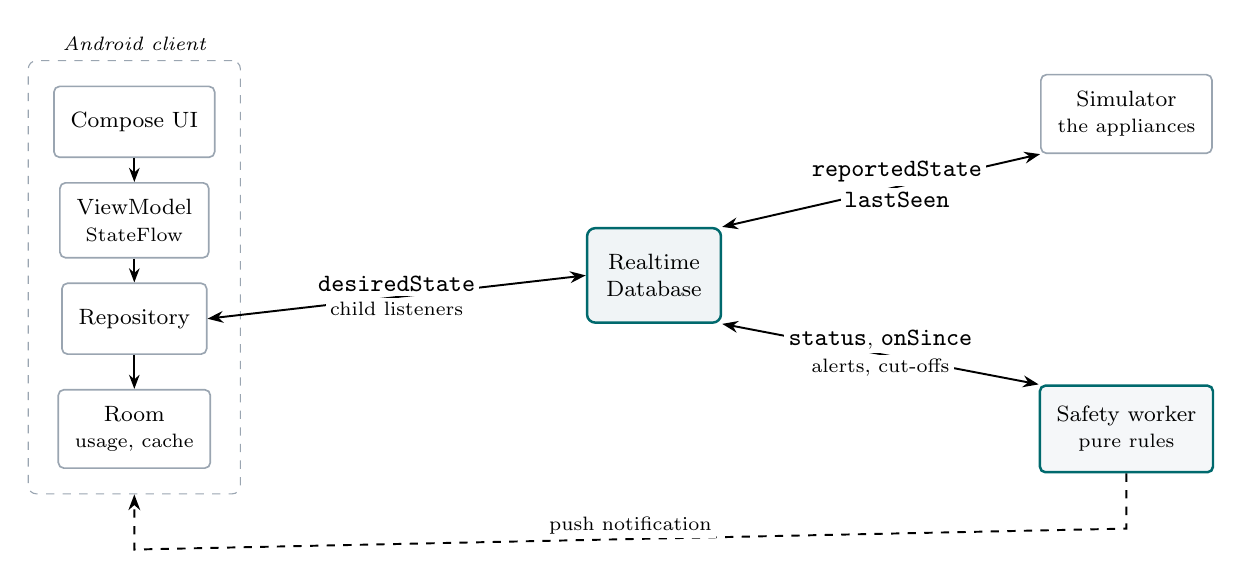
\begin{tikzpicture}[
    font=\footnotesize,
    box/.style={draw=rule,fill=white,line width=0.6pt,rounded corners=2pt,
                inner sep=6pt,align=center,minimum height=9mm},
    db/.style={draw=accent,fill=boxbg,line width=0.9pt,rounded corners=3pt,
               inner sep=7pt,align=center,minimum height=12mm},
    worker/.style={draw=accent,fill=codebg,line width=0.9pt,rounded corners=2pt,
                   inner sep=6pt,align=center,minimum height=11mm},
    flow/.style={{Stealth[length=2mm]}-{Stealth[length=2mm]},line width=0.7pt},
    push/.style={-{Stealth[length=2mm]},line width=0.7pt,dashed},
    lbl/.style={font=\scriptsize,align=center,fill=white,inner sep=1.5pt}
  ]

  % phone stack
  \node[box] (ui)   at (0,2.5)  {Compose UI};
  \node[box] (vm)   at (0,1.25) {ViewModel\\\scriptsize StateFlow};
  \node[box] (repo) at (0,0)    {Repository};
  \node[box] (room) at (0,-1.4) {Room\\\scriptsize usage, cache};

  \draw[-{Stealth[length=1.8mm]},line width=0.6pt] (ui) -- (vm);
  \draw[-{Stealth[length=1.8mm]},line width=0.6pt] (vm) -- (repo);
  \draw[-{Stealth[length=1.8mm]},line width=0.6pt] (repo) -- (room);

  \begin{scope}[on background layer]
    \node[draw=rule,dashed,rounded corners=3pt,inner sep=9pt,
          fit=(ui)(vm)(repo)(room),label={[font=\scriptsize\itshape,
          anchor=south]above:Android client}] (phone) {};
  \end{scope}

  % database
  \node[db] (dbn) at (6.6,0.55) {Realtime\\Database};

  % simulator and worker
  \node[box] (sim) at (12.6,2.6) {Simulator\\\scriptsize the appliances};
  \node[worker] (wk) at (12.6,-1.4) {Safety worker\\\scriptsize pure rules};

  % flows
  \draw[flow] (repo.east) -- node[lbl,above]{\code{desiredState}}
                             node[lbl,below]{child listeners} (dbn.west);
  \draw[flow] (sim.south west) -- node[lbl,above,pos=0.45]{\code{reportedState}}
                                  node[lbl,below,pos=0.45]{\code{lastSeen}} (dbn.north east);
  \draw[flow] (wk.north west) -- node[lbl,above,pos=0.5]{\code{status}, \code{onSince}}
                                 node[lbl,below,pos=0.5]{alerts, cut-offs} (dbn.south east);

  \draw[push] (wk.south) -- ++(0,-0.7) -- node[lbl,above]{push notification}
              ($(phone.south)+(0,-0.7)$) -- (phone.south);

\end{tikzpicture}
\caption{Component arrangement. Each process writes a disjoint set of fields,
and the database security rules enforce the separation.}
\label{fig:architecture}
\end{figure}

Four rules are evaluated against every device, as summarised in Table
\ref{tab:rules}.

\begin{table}[h]
\centering
\caption{Rules evaluated by the safety worker}
\label{tab:rules}
\begin{tabular}{@{}L{4.6cm}L{9.5cm}@{}}
\toprule
\textbf{Rule} & \textbf{Function} \\
\midrule
\code{maxOnDurationRule}    & Sets \code{desiredState} to false, appends a \code{CUTOFF} usage event, raises a critical alert and sends a push notification \\
\code{statusRule}           & Derives \code{status} and maintains \code{onSince} and \code{mismatchSince} \\
\code{staleHeartbeatRule}   & Marks a device disconnected when its heartbeat exceeds fifteen seconds \\
\code{scheduleRule}         & Applies on and off transitions at configured minute boundaries \\
\bottomrule
\end{tabular}
\end{table}

\subsection{Persistence of timer state}

Timer state is held in the database rather than in process memory. The field
\code{onSince} is stored, and elapsed time is recomputed from it at every
evaluation.

\begin{lstlisting}[language=,caption={The cut-off condition, abridged from
\code{worker/src/rules/maxOnDurationRule.ts}},label={lst:cutoff}]
const elapsedSeconds = Math.floor((clock.now() - slot.onSince) / 1000);
if (elapsedSeconds < limitSeconds) continue;
// Elapsed time is derived from stored state, not from a timer held in memory.
\end{lstlisting}

A timer implemented with \code{setTimeout} would be lost if the process
terminated, and would be lost without any indication that it had been. Because
the state is stored, a worker that crashes, is redeployed or loses power resumes
correctly: the next evaluation observes an appliance that has been running for
forty-seven seconds against a thirty-second limit and switches it off
immediately. This scenario is covered by a unit test, as is the requirement that
the cut-off fire at exactly \code{max\_on\_duration}.

Two triggers drive the same evaluation function. Child listeners provide
immediate reaction to changes, and a thirty-second sweep guarantees recovery
after any interruption. Since both invoke the identical function, they cannot
produce inconsistent results.

\subsection{Schedule semantics}

The schedule rule acts on transitions rather than on intervals: it applies a
change at the configured on-minute and off-minute only. Enforcing the interval
continuously would override manual control, so that a user switching a scheduled
light off at 19:00 would find it switched on again within a minute. Acting only
at boundaries allows a manual override to persist until the next boundary.

Rule application is idempotent, since at a boundary minute a write occurs only
when \code{desiredState} differs from the target value. The sweep therefore
cannot apply a transition twice. The consequence of this design is that a
boundary occurring entirely while the worker is unavailable is not applied
retrospectively.

% ============================================================================
\appendix
\newpage
\section{Architecture and technology}
\label{app:architecture}

The application is written in Kotlin using Jetpack Compose with Material 3,
following the MVVM pattern: composable functions observe a ViewModel exposing
\code{StateFlow}, which depends on a repository, which depends on the data
sources. No composable function accesses Firebase or Room directly. The minimum
supported API level is 26 and the target is 35. The build uses the Gradle Kotlin
DSL with a version catalogue.

Dependency injection is performed manually. For an application with a single
repository, a dependency injection framework would add a further component to be
understood and defended without corresponding benefit.

Two product flavours are provided. The \code{live} flavour communicates with
Realtime Database. The \code{demo} flavour runs against an in-memory
implementation that performs the roles of simulator, worker and database,
including a functioning safety cut-off, and therefore exercises the real
repository, ViewModels and interface without network access.

Room is not required by the specification. It is used for offline availability
and because the reporting screen aggregates usage in SQL rather than in
application code over a database snapshot.

\section{Verification}
\label{app:verification}

\begin{table}[h]
\centering
\caption{Automated test coverage}
\begin{tabular}{@{}L{4.2cm}L{1.8cm}L{8.0cm}@{}}
\toprule
\textbf{Suite} & \textbf{Tests} & \textbf{Coverage} \\
\midrule
Application unit tests & 73 & Grid mapping, wire format, repository propagation, Room aggregation, CSV escaping, schedule windows \\
Worker rule tests      & 40 & Cut-off timing under a controlled clock, restart recovery, status precedence, schedule boundaries \\
\midrule
\textbf{Total}         & \textbf{113} & \\
\bottomrule
\end{tabular}
\end{table}

Both \code{./gradlew assembleDebug} and \code{./gradlew test} complete
successfully, as do \code{npm test} and type checking in the worker project. A
continuous integration workflow runs both suites on every push from a checkout
containing no credentials.

\section{Requirement traceability}
\label{app:traceability}

Each requirement is mapped to its implementation, its verification, and the
point in the demonstration recording at which it is shown. Requirements marked
\textbf{M} describe integration behaviour spanning a mobile device, a browser and
a server process, and are verified by demonstration rather than by automated
test.

\begin{longtable}{@{}L{0.8cm}L{4.6cm}L{4.2cm}L{3.1cm}L{1.1cm}@{}}
\toprule
\textbf{\#} & \textbf{Requirement} & \textbf{Implementation} & \textbf{Verification} & \textbf{Demo} \\
\midrule
\endfirsthead
\toprule
\textbf{\#} & \textbf{Requirement} & \textbf{Implementation} & \textbf{Verification} & \textbf{Demo} \\
\midrule
\endhead
R1  & Multiple floor plans, added and managed & \code{ui/floors/} & Repository tests & 4:30 \\
R2  & Abstract grid mapping over layouts & \code{ui/plan/GridMapper.kt} & \code{GridMapperTest}, 16 tests & 2:15 \\
R3  & Sample plans supplied & \code{FloorPlanSpec.kt} & Compose preview & 2:15 \\
R4  & Toggling reactively updates the interface & \code{ui/device/}, \code{DeviceViewModel} & Repository tests & 6:00 \\
R5  & Four operational states displayed & \code{Slot.kt}, \code{StatusPill.kt} & \code{SlotTest}, worker tests, previews & 2:45 \\
R6  & Outlets as single-node binaries & \code{DeviceKind.OUTLET} & \code{WireTest} & 6:00 \\
R7  & Multi-switch as a single entity & \code{Device.kt} & \code{SlotTest}, repository tests & 5:00 \\
R8  & \code{max\_on\_duration} on hazard slots & \code{maxOnDurationRule.ts} & Worker tests, exact timing & 8:30 \\
R9  & Lights on preset time periods & \code{scheduleRule.ts} & \code{ScheduleTest}, worker tests & 7:45 \\
R10 & Cameras with simulated streams & \code{CameraCard.kt} & Compose previews & 9:30 \\
R11 & Client changes reach the database & \code{RealtimeDatabaseSource.kt} & Repository tests & 6:00 \\
R12 & External changes reach the client & \code{callbackFlow} listeners & Repository tests & 11:00 \\
R13 & Server-side cut-off & \code{maxOnDurationRule.ts} & Worker tests, live run & 15:30 \\
R14 & Cut-off raises an alert & \code{notifications.ts}, \code{ui/alerts/} & Demonstration \textbf{(M)} & 15:30 \\
R15 & Usage reporting & \code{ui/report/}, \code{UsageDao} & \code{UsageDaoTest} and others & 18:00 \\
R16 & Web simulator reflecting updates & \code{simulator/index.html} & Demonstration \textbf{(M)} & 10:30 \\
R17 & Simulator listens to the database & \code{simulator/index.html} & Demonstration \textbf{(M)} & 6:00 \\
D1  & Repository and APK & \code{apk/HomeSense-1.0.apk} & Signature verified & --- \\
D2  & Technical report & This document & --- & --- \\
D3  & Demonstration, three members & Demonstration script & --- & 0:00 \\
\bottomrule
\end{longtable}

\section{Limitations}
\label{app:limitations}

\textbf{Client roles are not distinguished.} The mobile client and the simulator
both authenticate anonymously, so the security rules cannot separate them. A
modified client could write \code{reportedState} as though it were hardware.
Separating the two roles would require custom authentication claims and a
service to issue them, which is outside the scope of this assignment. No client
can write \code{status}, which is the property on which the safety argument
depends.

\textbf{A single home is supported.} The database tree is keyed by home
identifier, so support for multiple homes would be additive, but it is not
implemented.

\textbf{The worker must be running.} If the worker stops, no status is derived,
no cut-off occurs and no schedule is applied. This is a single point of failure.
The simulator therefore displays the worker's own heartbeat and reports when it
is not running.

\textbf{Camera feeds are simulated,} as the specification permits. Frames are
generated locally. The configured snapshot and stream URIs are displayed beneath
the tile so that the mechanism a real camera would use remains visible.

\textbf{Energy figures are estimates.} They assume the rated wattage is drawn
for the whole period during which an appliance is on, and are labelled as
estimates wherever they appear.

\section{Design decisions}
\label{app:adr}

\begin{table}[h]
\centering
\begin{tabular}{@{}L{1.2cm}L{13.3cm}@{}}
\toprule
\textbf{Ref} & \textbf{Decision} \\
\midrule
0001 & Realtime Database in preference to Firestore, for per-child listeners and \code{onDisconnect()} \\
0002 & Android Gradle Plugin 8.13.2 with compileSdk 36, since current androidx releases require AGP 9 and a correspondingly recent Android Studio \\
0003 & A standalone Node worker in preference to Cloud Functions, which require a billing plan; the rules remain portable to Cloud Functions unchanged \\
\bottomrule
\end{tabular}
\end{table}

\end{document}
